\title{Reti Peer to Peer}
\maketitle

\chapter{Kademlia}
\section{Introduzione}
Kademlia è un \textbf{DSM-based protocol}, specifica la struttura della rete, le regole di comunicazione tra i nodi e il modo in cui l'informazione viene scambiata. \'E basata sulla tecnologia \textbf{Distributed Hash Table (DHT)}, dove ogni risorsa pubblicata è associata a una \textbf{coppia <chiave,valore>}. Il valore potrebbe essere la risorsa propria o solo un suo descrittore. La chiava è di solito un hash del descrittore di risorsa. 

\section{Distanza tra identificatori}
Kademlia usa chiavi a 160 bit per identificare risorse e nodi. Nella fase di pubblicazione, la coppia chiave$-$valore associata alla risorsa è assegnata al nodo il cui identificatore è il più vicino rispetto alla chiave della risorsa. La metrica adottata è basata sull'operazione logica \textbf{XOR}.

Siano X e Y due identificatori: 
\[
d(X,Y) = X \oplus Y
\]
Esempio: la distanza tra 010101 e 110001 è 100100, cioè 36.

Caratteristiche della matrica XOR:
\begin{itemize}
    \item $d(X,X) = 0$
    \item $d(X,Y) > 0$ se $X \neq Y$ 
    \item $d(X,Y) = d(Y,X)$ per qualsiasi X,Y
    \item $d(X,Y) + d(Y,Z) \geq d(X,Z)$
\end{itemize}
La matrica è unidirezionale cioè per una qualsiasi X e distanza $\Delta > 0$ c'è un'unica Y tale che $d(X,Y) = \Delta$. 

\section{Strutture dati nodi}
Ogni nodo ha \textbf{160 k-buckets}. Un k$-$bucket è una lista di (massimo k) $<$indirizzi IP, porta UDP, Node ID$>$ tuple correlate ai nodi le cui distanze dal nodo corrente sono contenute tra $2^i$ e $2^{i+1}$ (con i tra 0 e 159). Ogni k$-$bucket è ordinato come segue: dalla testa, il nodo contattato meno di recente, alla coda, quello più recente. 
\begin{center}
    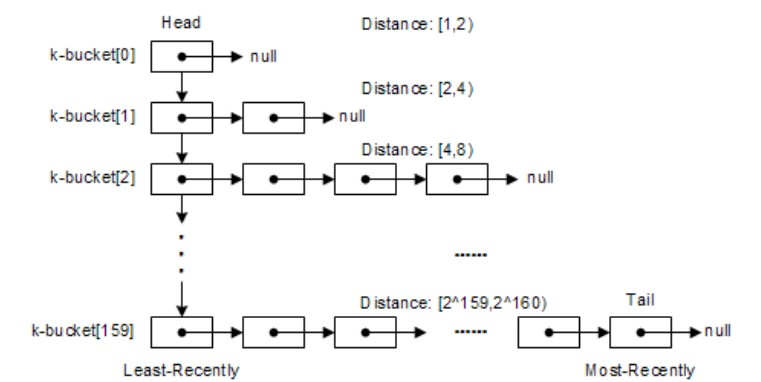
\includegraphics[scale = 0.4]{Images/P2P/KademliaNodeStructure.jpg}
\end{center}
Quando un nodo riceve un messaggio da un altro nodo, controlla il k$-$bucket che dovrebbe contenere il descrittore del mittente. Se il descrittore è trovato, il nodo lo muove alla coda del bucket, altrimenti il nodo lo aggiunge alla coda del bucket. Se il bucket è pieno, il nodo manda un messaggio PING al nodo il cui descrittore è locato in testa al bucket (il nodo visto meno recentemente). Se non si ottiene nessuna risposta, il descrittore del nodo contattato è rimosso dal bucket e uno dei nuovi nodi è aggiunto alla coda del bucket. Altrimenti, questo descrittore del nuovo nodo è scartato. 

\textbf{Perché privilegiare i nodi disponibili da lungo tempo rispetto ai nuovi arrivati?} Si ricorda la lunghezza di vita dei nodi in Gnutella e Shifted Pareto, che sono caratterizzati da E[R] $>$ E[L]. 

\section{Protocollo RPCs}
Il protocollo di Kademlia consiste di 4 RPCs:
\begin{itemize}
    \item PING: Il nodo n1 invoca PING sul nodo n2 per verificare che quest'ultimo sia online
    \item STORE: n1 invoca STORE($<$chiave, valore$>$) sul nodo n2 per fargli memorizzare la copia passata
    \item FIND\_NODE: n1 invoca FIND\_NODE($<$chiave$>$) sul nodo n2 per ottenere i descrittori $<$indirizzo IP, porta UDP, Node ID$>$ dei \textbf{k} nodi nel k$-$bucket di n2 che sono i più vicini alla chiave richiesta. Tali descrittori possono venire dallo stesso k$-$bucket o da diversi, se il primo considerato non è completo
    \item FIND\_VALUE: come FIND\_NODE con la seguente eccezione: se n2 è stato precedentemente richiesto per eseguire una STORE con la stessa chiave allora n2.FIND\_VALUE($<$chiave$>$) ritorna il valore associato a quella chiave
\end{itemize}


\section{Ricerca ricorsiva dei nodi}
Il nodo n seleziona $\alpha$ nodi dal k$-$bucket che è il più vicino a un identificatore specifico X. Se tale k$-$bucket non contiene $\alpha$ nodi, il nodo n prende gli $\alpha$ nodi i cui ID è il più vicino a X, tra quelli che n conosce. Successivamente, n invoca FIND\_NODE(X) sugli $\alpha$ nodi selezionati, in parallelo. 

Dai risultati ottenuti, il nodo n prende i k nodi che sono i più vicini a quello con identificatore X, Tra questi nodi, il nodo n prende $\alpha$ nodi ai quali non è stato ancora richiesto e invoca FIND\_NODE(X) su loro, in parallelo. 

Questo processo è ripetuto ricorsivamente. Se un round di FIND\_NODE non ritorna alcun nodo vicino rispetto al target, il nodo n invoca FIND\_NODE(X) sugli altri $k-\alpha$ nodi (dal k$-$set dei nodi più recentemente ottenuto). Il processo si ferma quando il nodo n ha (con successo) chiesto tutti i k nodi più vicini al target.

\section{Principio principale di Kademlia}
Intuizione geometrica: la distanza tra nodi dello stesso sottoalbero è più piccola di quella tra nodi di sottoalberi diversi. Kademlia si basa su questo principio. Ad ogni nuovo passo verso il target, il numero di possibili candidati si dimezza (in teoria).
\begin{center}
    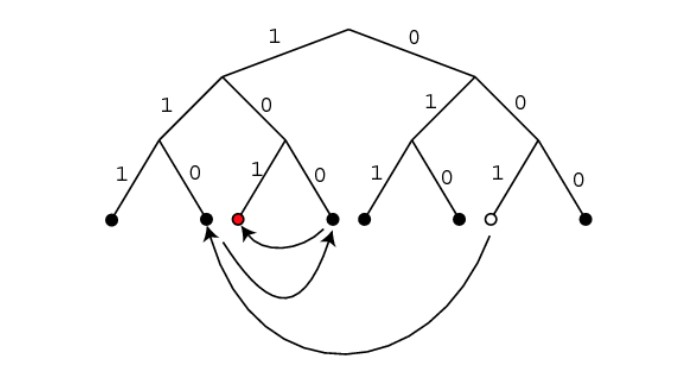
\includegraphics[scale = 0.4]{Images/P2P/MainPrincipleKademlia.jpg}
\end{center}
In Kademlia, la ricerca del nodo illustrata sopra è la base per la risorsa
meccanismi di pubblicazione e ricerca. 

Per \textbf{pubblicare un descrittore di risora} (coppia chiave valore in cui il valore è il descrittore e la chiave è il suo hash) il nodo n cerca i k nodi più vicini rispetto alla chiave della risorsa. Dopodichè, n invoca STORE(<chiave,valore>) su loro.

La \textbf{ricerca per una coppia <chiave,valore>} lavora allo stesso modo: il nodo n cerca i k nodi più vicini rispetto alla chiave della risorsa. Dopodichè, n invoca FIND\_VALUE(<chiave>) su loro.\\

Sia la pubblicazione che la ricerca sono caratterizzate da tempo di esecuzione O($\log_2N$), dove \emph{N} è il numero di nodi nella rete. $\log_2N$ è la altezza dell'albero binario illustrato sopra. 

\section{Connessione a Kademlia}
Ogni nodo n1 che si aggiunge alla rete, lo fa attraverso un nodo conosciuto n2. Il nodo n1 inserisce n2 nel k$-$bucket più adatto, dopodichè inizia una ricerca di nodo con la propria chiave come parametro. In questo modo n1 popola il suo k$-$bucket e notifica la sua presenza a tutti i nodi contattati. \\

Il condizioni a regime:
\begin{itemize}
    \item la tabella di routing di ogni nodo contiene i k nodi più vicini
    \item un k$-$bucket è vuoto se e solo se nella rete non ci sono nodi con ID che "cade" in quel bucket
    \item la probabilità che un nodo sia contattato da un nodo a una distanza tra $2^i$ e $2^{i+1}$ è costante e indipendente dal valore di i (che è compreso tra 0 e 159)
\end{itemize}


\chapter{Skype}
\section{Introduzione}
Caratteristiche:
\begin{itemize}
    \item Basato sul \textbf{peer-to-peer LM}, l'unico elemento centralizzato è il server di login
    \item Permette firewall e NAT trasversali, grazie ai supernodi
    \item Offre una qualità vocale maggiore dei competitor: trasmette con UDP a 36Kbps e l'audio è compresso tramite codec \textbf{iLBC}
\end{itemize}


\section{Registrazione}
L'utente decide il proprio \textbf{username A} e la propria \textbf{password P$_A$}. Da (A, P$_A$), il peer dell'utente genera \textbf{una coppia di chiavi RSA (S$_A$, V$_A$)}, dove \textbf{S$_A$ è la chiave privata di firma} e \textbf{V$_A$ è la chiave pubblica di verifica}. Il peer utente memorizza S$_A$ e \textbf{H(P)}$_A$ in una cache locale sicura. 

Il peer utente e il server di login stabiliscono una sessione basata su \textbf{AES} con chiave di 256 generata randomicamente e codificata con \textbf{V}$_{LS}$ prima di essere mandata al server dal peer utente. Il peer utente manda \textbf{A}, \textbf{V}$_A$ e \textbf{H(P)}$_A$ al server di login. Il server controlla che A non sia un username già esistente. Se il controllo ha successo, il server:
\begin{itemize}
    \item salva A e H(H(P$_A$)) in un database
    \item crea un \textbf{certificato di identità IC}$_A$ \textbf{contenente (A, V}$_A$)$^{S_{LS}}$ e lo manda al peer utente
\end{itemize}
In questa fase, il server di login si comporta come una \textbf{certification authority}, fornendo al peer utente un certificato da usare per autenticarsi con gli altri peers e al server stesso. 

\section{Login}
Il peer utente si autentica (con il suo IC) al login server, che gli fornisce una lista di \textbf{supernodi}. I supernodi sono peer con IP pubblico e risorse sufficienti per servire poche migliaia di peer \textbf{foglie}. Il peer utente seleziona un supernodo e apre una connessione TCP con lui. Inoltre, si annuncia ai membri della sua \textbf{buddy list}. La ricerca di altri peer è basata sullo scambio di messaggi tramite supernodi. Il peer utente è in grado di identificate il tipo di NAT, nel caso ci sia. 

\begin{center}
    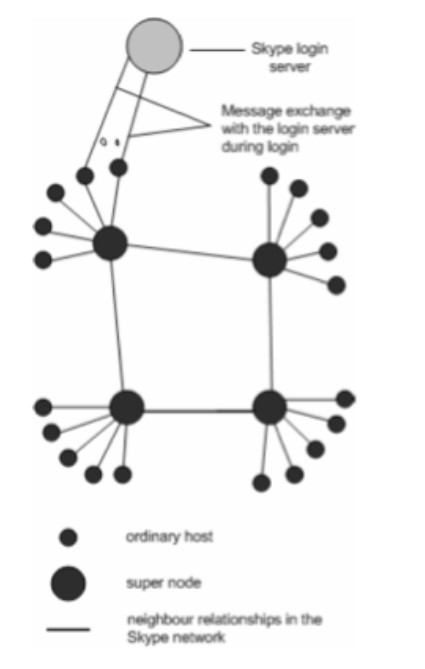
\includegraphics[scale = 0.4]{Images/P2P/Skype.jpg}
\end{center}

\section{Chiamate e comunicazioni}
Il segnali di inizio e fine chiamata sono sempre mandati tramite TCP, direttamente tra peer A e peer B, o per mezzo di uno o più supernodi. I due peer adottano il seguente \textbf{protocollo di accordo di chiave}:
\begin{enumerate}
    \item scambio di pacchetti di 64 bit, firmati con la chiave privata e verificati dal ricevitore usando la chiave pubblica del mittente
    \item autenticazione mutua basata sullo scambio di IC
    \item creazione di \textbf{chiavi di sessione SK}$_{AB}$ \textbf{di 256 bit}, ogni bit contribuisce con 128 bit, negoziazione basata su RSA
\end{enumerate}
\textbf{La comunicazione è basata su UDP, usando AES con la chiave di sessione SK}$_{AB}$. In questo modo, anche se la comunicazione è instradata dai supernodi, solo il mittente e il ricevitore possono decifrare i pacchetti.


\chapter{WebRTC e PeerJS}
\section{Introduzione a webRTC}
WebRTC è un progetto aperto e gratuito che fornisce browser e applicazioni mobili con funzionalità di \textbf{comunicazioni in tempo reale (RTC)} tramite semplici API. I componenti WebRTC sono stati ottimizzati per servire al meglio questo scopo. WebRTC offre agli sviluppatori di applicazioni web la possibilità di scrivere contenuti ricchi, applicazioni multimediali in tempo reale (es. chat video) sul web, senza richiedere plug-in, download o installazioni.
Il suo scopo è aiutare a costruire una solida piattaforma RTC che funzioni
più browser Web, su più piattaforme.

\begin{center}
    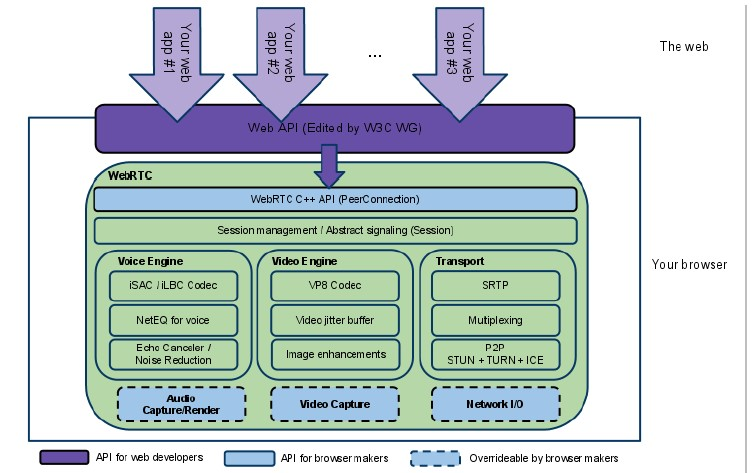
\includegraphics[scale = 0.4]{Images/P2P/ArchitetturaWebRTC.jpg}
\end{center}

\subsection{No plugins}
Molte web application usano già RTC ma necessitano di downloads, app native o plugins. Scaricare, installare e aggiornare plugins può essere molto complesso, propenso a errori e fastidioso. I plugin, inoltre, possono essere difficili da distribuire, debuggare, trovare errori, testare e mantenere e potrebbero richiedere licenze e integrazioni con tecnologie complesse e costose. \'E spesso difficile convincere persone a installare plugins.

\subsection{Applicazioni WebRTC}
Applicazioni webRTC necessitano di fare molte cose:
\begin{itemize}
    \item Ottenere/fornire \textbf{streaming} audio, video
    \item Ottenere \textbf{informazioni di rete} come gli indirizzi IP e porte e scambiare queste con altri client webRTC (peers) per abilitare la connessione, anche attraverso NAT e firewalls
    \item Coordinare \textbf{comunicazioni di segnalazioni} per segnalare errori e iniziare sessioni di chiusura
    \item Scambiare informazioni su media e \textbf{capacità} dei client, come la risoluzione e codec
\end{itemize}

\subsection{API di webRTC}
WebRTC ha diverse \textbf{javascript API}:
\begin{itemize}
    \item MediaStream aka getUserMedia(): cattura audio e video
    \item RTCPeerConnection: stream audio e video tra utenti
    \item RTCDataChannel: strean dati tra utenti
\end{itemize}

\subsection{STUN e TURN}
WebRTC è progettato per lavorare peer$-$to$-$peer in modo che gli utenti possano essere connessi dal percorso più diretto possibile. Tuttavia, webRTC è costruito per avere a che fare con il networking reale: applicazioni client necessitano di \textbf{traverse NAT gateways e firewall}, e networking peer$-$to$-$peer necessita di alternative nel caso la connessione diretta fallisca. Come parte di questo processo, le API di webRTC usano \textbf{server STUN per ottenere l'indirizzo IP del tuo computer}, e \textbf{server TURN per funzionare come server staffetta} nel caso la connessione peer$-$to$-$peer fallisca.


\subsection{Sicurezza}
La \textbf{cifratura} è obbligatoria per tutte le componenti webRTC, e le sue API javascript possono essere usate solo da \textbf{origini sicure} (HTTPS o localhost).

\emph{The basic assumption of this architecture is that network resources
exist in a hierarchy of trust, rooted in the browser, which serves as
the user's Trusted Computing Base (TCB). Any security property which
the user wishes to have enforced must be ultimately guaranteed by the
browser (or transitively by some property the browser verifies).
Conversely, if the browser is compromised, then no security
guarantees are possible.}

La specifica webRTC assume che una volta che alla pagina web è stato dato il permesso di accedere ai media, è libera di condividere quel media con altre entità che sceglie.

\section{PeerJS}
PeerJS avvolge l'implementazione webRTC del browser per fornire una API di connessione peer$-$to$-$peer completa, configurabile e facile da usare. Equipaggiato solo con un ID, un peer può creare una connessione di dati o media stream a un peer remoto. \\

Nelle diapo fa vedere come si usa precisamente a livello di codice.\\

\subsection{PeerServer}
Per mediare le connessioni, PeerJS si connette a un PeerServer.
Si noti che nessun dato peer-to-peer passa attraverso il server; il server
funge solo da broker di connessione. 

PeerJS offre una versione gratuita di PeerServer ospitata nel cloud: https://peerjs.com/peerserver.html.
L'utente può eseguire il proprio PeerServer (è scritto in Node.js): https://github.com/peers/peerjs-server.